\documentclass[12pt]{book}

% Lingua e pacchetti principali
\usepackage[utf8]{inputenc}  % Codifica dei caratteri
\usepackage[english]{babel}  % Lingua italiana (puoi cambiarla con 'english' se preferisci l'inglese)
%\usepackage{amsmath, amssymb}  % Pacchetti matematici
\usepackage{graphicx}  % Inserimento immagini
\usepackage{fancyhdr}  % Per intestazioni personalizzate
\usepackage[colorlinks=true, linkcolor=black, urlcolor=blue, citecolor=black]{hyperref}
\usepackage{geometry}  % Personalizzazione dei margini

% Personalizzazione dei margini
\geometry{top=3cm,bottom=3cm,left=2.5cm,right=2.5cm}

% Inizio del documento
\begin{document}

% Frontespizio (titolo, autore, data, etc.)
\title{Il mio libro di trading}
\author{Fabio Rizzi}
\date{\today}
\maketitle  % Crea il frontespizio

% Sommario
\tableofcontents

% Parte introduttiva
\chapter*{Introduzione}
la semplicità nel trading è l'approccio migliore per ottenere buoni risultati.\\
Utilizzare pochi e semplici strumenti
% Capitolo 1
\chapter{Capitolo 1: Il concetto di Trading}
\section{Il trading} 
Attività di compravendita di strumenti finanziari, nel nostro caso Criptovalute. La variazione di prezzo, il risultato di questa attività.

Possiamo paragonare il trading alla battaglia tra la pressione d'acquisto dei compratori e quella di vendita dei venditori. Noi non possiamo conoscere l'esito della battaglia, possiamo solo prevederlo.

Analizzando con metodo logico la battaglia, aumentiamo la nostra probabilità di prevedere correttamente l'esito.
\section{Il grafico a candele} "fig. \ref{graficocandele}" Rappresenta visivamente l'andamento del prezzo nei diversi intervalli di tempo, noti come timeframe. Ogni candela simboleggia l'esito di una battaglia tra compratori e venditori: una candela verde indica che i compratori hanno prevalso sui venditori, mentre una candela rossa segnala la vittoria dei venditori sui compratori.

\begin{figure}[h!]
    \centering
    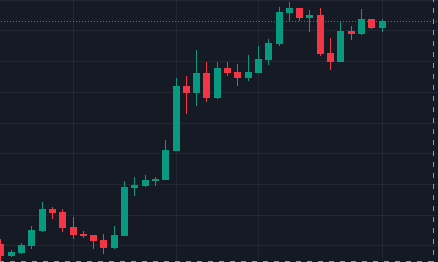
\includegraphics[width=0.5\linewidth]{Immagini/grafico-candele.png} % Nome del file immagine (senza estensione se è PDF, PNG, JPG)
    \caption{rappresentazione di grafico a candele giapponesi.}
    \label{graficocandele} % Etichetta per riferimento incrociato
\end{figure}



\section{Il trader} 
Osserva l'andamento del prezzo e studia le conformazioni che le candele disegnano nel grafico. Grazie alle conformazioni che si ripetono nel tempo, il trader formula una sua strategia che migliora la sua probabilità statistica nel prevedere l'andamento del prezzo.

\section{Gli strumenti di lavoro del trader}
\begin{description}
    \item[*] L'indice
    \item[*] Il grafico, le candele
    \item[*] Il book di negoziazione, il libro degli ordini
    \item[*] Le ema
    \item[*] La wvap
    \item[*] La trendline
    \item[*] I punti trigger
    \item[*] Le conformazioni
    \item[*] Il broker
\end{description}
%%%%%								CAPITOLI
\chapter{Capitolo 2 I grafici}

\section{Il grafico a candele}
Il grafico a candele è come una mappa, più informazioni fornisce, maggiori sono le possibilità di raggiungere la destinazione in sicurezza.  Saper leggere la mappa è fondamentale per aumentare la propria statistica.
Il grafico a candele rappresenta graficamente la forza della domanda e dell'offerta, l'andamento del mmercato, importanti indizi di inversione di trend.

\subsection{La psicologia del mercato.}
L'aspetto psicologico del mercato si riflette nel grafico a candele.
E' importante considerare le seguenti 3 regole:
\paragraph{regola nr 1}
Quando vedi una tendenza rialzista/ribassista,considerala un'opportunità di vendita/acquisto.
\paragraph{regola nr 2}
Quando senti notizie rialziste o ribassiste, non fare trading su di loro.
\paragraph{regola nr 3}
Non dire agli altri ciò che stai per fare nel mercato; prendi le tue decisioni solo guardando il mercato.

\subsection{La candela}
Composta da una sezione rettangolare e due linee sottili sopra o sotto registra il movimento del prezzo rispetto alla sessione temporale del grafico.
La sezione rettangolare è chiamata corpo reale e rappresenta l'intervallo di prezzo tra apertura e chiusura della sessione temporale, le singole linee sopra e sotto il corpo questa
sezione. Vediamo perché questi sono chiamati grafici a candela; le singole
linee spesso sembrano candele con i loro stoppini. La parte rettangolare della
linea delle candele è chiamata corpo reale. Rappresenta l'intervallo tra
l'apertura e la chiusura della sessione. Quando il corpo reale è nero (ad esempio, riempito),
mostra che la chiusura della sessione è stata inferiore all'apertura. Se il corpo reale è bianco (cioè, vuoto), significa che la chiusura è stata superiore all'apertura.
 
\section{le medie mobili}
\chapter{Capitolo 3 I grafici}

\section{Le candele}
%%%%%	
%\begin{equation}
%E = mc^2
%\end{equation}

% Sezione del Capitolo
%\section{Una Sezione}
%Questa è una sezione all'interno del capitolo. Puoi aggiungere sottosezioni e paragrafi come desideri.

% Capitolo 2
\chapter{L'indice}
Nel mondo Criptovalute Bitcoin è l'indice. Bitcoin detiene oltre il 70\% del market cup mondiale in criptovalute ed è considerato l'immacolata concezione delle criptovalute. 



% Bibliografia
\newpage
\chapter*{Bibliografia}
\addcontentsline{toc}{chapter}{Bibliografia}
\begin{thebibliography}{9}
\bibitem{latex} Donald E. Knuth, \textit{The TeXbook}, Addison-Wesley, 1986.
\end{thebibliography}

\end{document}
